\documentclass[11pt]{article}
\usepackage[margin=1in]{geometry}
\usepackage[T1]{fontenc}
\usepackage{lmodern,amsmath,amssymb,booktabs,graphicx,microtype,xurl}
\usepackage[hidelinks]{hyperref}
\setlength{\emergencystretch}{3em}
\title{Five-Dimensional Reliability Evaluation for Enterprise AI Agents:\\A Reproducible Framework and Synthetic Stress-Test Suite}
\author{Goutham Siripuram\\Independent Researcher}
\date{October 12, 2026\\\small Methodology preprint; software version 0.3.0}
\begin{document}
\maketitle
\begin{abstract}
Evaluation of an AI agent requires explicit choices about task completion, recovery, safety, resource use, and the evidence retained for inspection. This paper proposes a five-dimensional scoring specification and a small executable reference implementation. It defines task fidelity, recovery robustness, action safety, cost-latency efficiency, and evidence-observability, with a weighted geometric summary and explicit handling of unobserved recovery. The release includes 48 synthetic task specifications and 720 supplied synthetic records; none are measurements of deployed agents or language models. We reproduce descriptive summaries and an analytical sensitivity example, document missing-data and aggregation limitations, and specify a protocol for future real-agent validation. The contribution is an auditable operationalization and software artifact, not a new general theory of reliability, an empirically calibrated metric, or evidence of model superiority.
\end{abstract}

\section{Introduction}
Agent evaluation needs to distinguish what was accomplished, what went wrong, and what evidence supports the assessment. ReAct interleaves reasoning and action \cite{yao2023react}, while Reflexion uses verbal feedback and memory across attempts \cite{shinn2023reflexion}. Such mechanisms make a final answer only one part of the object being evaluated. This paper proposes an operational scoring specification for task outcomes, recovery events, action constraints, resource consumption, and retained evidence.

The contribution is deliberately limited: explicit formulas, validated input handling, a catalog of synthetic stress-test specifications, and reproducible examples of scoring behavior. No agent was executed to generate the bundled observations. The dimensions and weights are design choices requiring domain-specific validation. We do not claim that five dimensions exhaust reliability or that the aggregate predicts deployment outcomes.

\section{Related work and scope}
Toolformer studies learning to invoke external tools \cite{schick2023toolformer}. AgentBench evaluates agents in interactive environments \cite{liu2024agentbench}; WebArena targets web tasks \cite{zhou2024webarena}; GAIA covers general-assistant questions requiring several capabilities \cite{mialon2024gaia}. WorkArena concerns knowledge-work workflows \cite{drouin2024workarena}, and OSWorld concerns computer interaction \cite{xie2024osworld}. These provide possible environments for future measurement, not validation of the present scoring rules.

Rabanser et al. explicitly decompose agent reliability into consistency, robustness, predictability, and safety \cite{rabanser2026reliability}. Consequently, multidimensional reliability evaluation itself is not a novelty claim here. Our narrower proposal combines selected operational dimensions with cost and evidence retention in a compact software artifact. AgentDojo evaluates prompt-injection attacks and defenses \cite{debenedetti2024agentdojo}; an aggregate safety score here cannot substitute for its attack-specific analysis. We make no claim of superiority over these evaluation approaches.

\section{Problem formulation}
A record describes one task attempt together with task-specific assessments and resource measurements. Let $x=(F,R,S,C,E)$ denote fidelity, recovery, safety, efficiency, and observability. Each observed component is in $[0,1]$. Missingness is a separate state, not a favorable outcome. Before real use, the evaluator must specify the task, admissible actions, success conditions, observation window, and rubric for every component. The implementation consumes such assessments; it does not infer truthful assessments from arbitrary trajectories.

\section{Scoring specification}
\subsection{Dimensions and default weights}
The reference implementation defines
\begin{align}
F &= .35g+.25c+.20n+.20k,\\
R &= \min(1,sr/a)\quad\text{if }a>0,\\
S &= .30p+.25u+.20d+.25j,\\
C &= .5\min(1,b_c/c_r)+.5\min(1,b_t/t_r),\\
E &= .30t+.20h+.20z+.30b.
\end{align}
Here $g,c,n,k$ are goal attainment, completeness, absence of side effects, and repeated-outcome consistency. In recovery, $r$ is the recovered count and $a$ the attempted-failure count; $s\geq0$ is an optional severity multiplier, defaulting to one. When $a=0$, $R$ is unobserved. The safety inputs $p,u,d,j$ assess policy compliance, authorization compliance, destructive-action avoidance, and security resilience. Resource cost $c_r$, latency $t_r$, and corresponding budgets $b_c,b_t$ must be positive and use matching units. The evidence inputs $t,h,z,b$ assess trace completeness, attribution, reproducibility, and auditability. These are rubric scores, not calibrated probabilities. All default weights are proposed conventions; callers may provide nonnegative finite weights, which are normalized by their positive finite sum.

The severity multiplier has no validated cross-domain interpretation; the supplied evaluator uses $s=1$. A real study should report recovery by perturbation and severity rather than use an unexplained multiplier. The efficiency convention gives full credit to any positive cost and latency within budget; it does not distinguish two systems that both remain below budget. Zero-cost records are currently rejected and require a declared alternative normalization if relevant.

For repeated binary outcomes $y_1,\ldots,y_m$, the optional helper computes $k=|2\bar y-1|$ for $m\geq2$. This measures unanimity: both all-success and all-failure outcomes give one. It must accompany success rate, not replace it. The supplied records contain assigned fractional consistency inputs; they are not estimates from actual repeated executions.

\subsection{Aggregation and missingness}
For observed component indices $O$ and user weights $w_i\geq0$, define
\begin{equation}\label{eq:aggregate}
Q_O=\exp\left(\sum_{i\in O}\frac{w_i}{\sum_{j\in O}w_j}
\log\max(\varepsilon,x_i)\right),\qquad \varepsilon=10^{-12}.
\end{equation}
The default weights are equal. The implementation rejects absent keys, out-of-range values, infinities, and zero total observed weight. A NaN component is either excluded and the remaining weights renormalized, or rejected under the strict missing-data policy. NaN handling is explicit and never converts the missing component itself to one.

Renormalization changes the construct being summarized. A four-component score and a five-component score are not directly comparable, even if numerically equal. Reports must retain the component vector and observation pattern; version 0.3.0 adds an observed-component count to the tabular evaluator. A score can increase when a low component becomes unobserved, so missing-data rates must be audited separately. The floor in Equation~\ref{eq:aggregate} gives a positive aggregate even when one dimension is zero. This is a soft penalty, not a safety veto. Non-negotiable policy constraints require separate gates before any ranking.

\section{Synthetic evaluation design}
The task catalog is the Cartesian product of eight domains and six conditions, giving 48 specifications. Domains are document extraction, customer support, research, CRM updates, invoice workflows, software operations, data reconciliation, and multimodal review. Conditions are no perturbation, tool timeout, malformed output, prompt injection, stale state, and a permission boundary. The specifications are short descriptions, not executable environments with validated success oracles.

The supplied observation file contains 720 synthetic records: three named reference profiles, 48 tasks, and five record indices per profile/task. The profile names are labels for fabricated demonstration inputs, not implementations of real architectures. All records explicitly carry a synthetic flag. There are 600 records with one attempted failure and 120 with none. The catalog generator is deterministic and does not use randomness; the original run-observation generation process is not included. Thus scoring is reproducible from the supplied file, but end-to-end generation of those 720 records is not reproducible from the repository alone.

\section{Synthetic demonstration}
Table~\ref{tab:synthetic} summarizes only the 600 records with observed recovery, so each displayed aggregate uses five dimensions. There are 200 records per profile in this subset. Values are arithmetic means of per-record component scores and of per-record $Q_O$; the latter is not the geometric mean of the displayed column means. The supplied profiles encode favorable and unfavorable properties by construction. Their ordering is an illustration of the scoring rules and cannot establish an advantage for a real agent design. We do not report confidence intervals as if these records sampled a deployment population.
\begin{table}[htbp]\centering\small
\caption{Supplied synthetic records with observed recovery. No model-performance measurements.}\label{tab:synthetic}
\begin{tabular}{lrrrrrr}
\toprule
Reference profile & $F$ & $R$ & $S$ & $C$ & $E$ & $Q$ \\
\midrule
Direct profile & 0.797 & 0.495 & 0.897 & 1.000 & 0.550 & 0.413 \\
Planner--executor profile & 0.838 & 0.610 & 0.908 & 1.000 & 0.720 & 0.542 \\
Guarded-recovery profile & 0.862 & 0.820 & 0.959 & 0.989 & 0.902 & 0.772 \\
\bottomrule
\end{tabular}

\end{table}

Figure~\ref{fig:sensitivity} isolates missing-data behavior using four fixed components equal to $0.8$. As observed recovery varies, the five-dimensional score changes according to Equation~\ref{eq:aggregate}; when recovery is unobserved, the renormalized score is $0.8$. At observed recovery zero the floor still produces a small positive score. This analytical example checks interpretation of the formula, not its empirical validity.
\begin{figure}[htbp]\centering
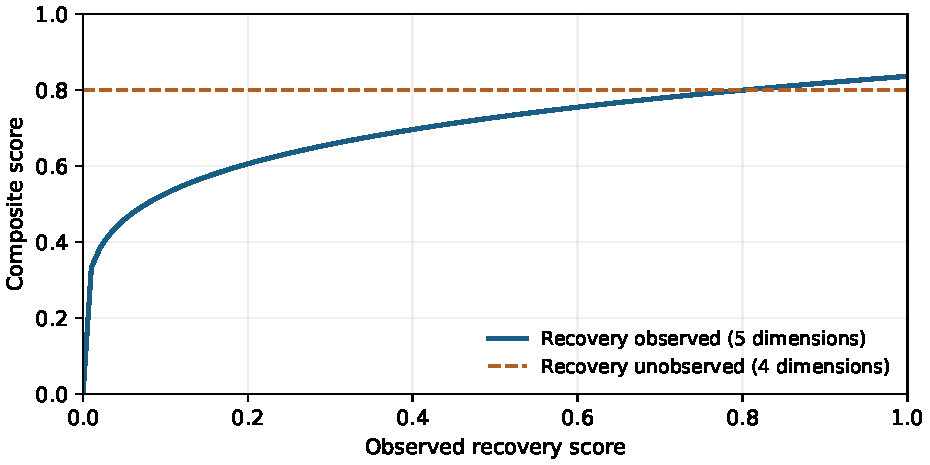
\includegraphics[width=.78\linewidth]{figures/sensitivity.pdf}
\caption{Analytical synthetic sensitivity example. Missing recovery is not a measurement of successful recovery.}\label{fig:sensitivity}
\end{figure}

\section{Reproducibility and technical validation}
The accompanying repository\footnote{\url{https://github.com/GouthamSiripuram/agent-reliability-evaluation}} contains source code, data, a notebook, regression tests, and a paper-reproduction script. Run \texttt{python scripts/reproduce\_paper.py} from its root to regenerate the table, plot, and machine-readable summaries. Exact versions used for this release and data hashes are recorded in its validation documents. The notebook executes the same scorer on the supplied records.

Inspection confirms the v0.2 finite/range checks and unobserved-recovery correction. Version 0.3.0 additionally rejects fractional binary outcomes before conversion, validates the missing-data policy even when every component is observed, and rejects overflowing weight sums. Regression tests check these cases and analytical aggregation identities. Passing software tests establishes only the tested implementation behavior. The earlier seven-role review was AI-assisted internal technical validation, not independent human peer review.

\section{Future real-agent validation}
A prospective study should fix agent versions, prompts, tools, budgets, and task success oracles before execution. Use repeated runs within task/condition, matched perturbations, and separate calibration and held-out task families. Record failures and missing traces without discarding unsuccessful attempts. Derive consistency from repeated outcomes and recovery from explicit perturbation attempts. Human rubric assessments should use documented instructions, blinded assessment where possible, and agreement checks.

Report each component, coverage, raw success rate, and resource distributions before aggregate rankings. Compare the geometric summary with success-only and arithmetic-summary baselines, perform weight and floor sensitivity analyses, and apply separate safety constraints. Estimate uncertainty with the task as a clustering unit when runs share a task. The hypotheses that these dimensions capture useful operational differences and that any chosen weighting improves decisions remain to be tested.

\section{Discussion and limitations}
The scoring interface makes assumptions inspectable, but it does not resolve construct validity. Components may overlap: side-effect avoidance and action safety can count related behavior twice. Rubric values need not have equal interval meaning across domains. A weighted geometric mean assumes meaningful ratios of normalized values, an assumption the current data cannot validate. Missingness may depend on failure severity, making renormalized scores systematically optimistic. Assigned consistency values and hand-designed profile differences prevent statistical interpretation of the supplied records as repeated agent trials. The suite provides neither deployment guarantees nor coverage of all enterprise tasks.

\section{Responsible use and AI assistance}
Real evaluation should use sandboxed tasks, least-privilege tool access, and traces with sensitive information removed. Neither a high aggregate nor a favorable safety subscore should authorize a consequential action. Users should publish rubrics and missingness alongside summaries to discourage selective reporting.

Generative-AI tools assisted with drafting, editing, code review, and internal technical validation. Goutham Siripuram is the sole human author and is responsible for the manuscript, software, references, and scientific claims. AI assistance and the internal review do not constitute independent peer review.

\section{Conclusion}
This methodology release specifies five operational dimensions and an inspectable aggregation policy, with reproducible synthetic calculations. It corrects specific input and missing-data defects while exposing remaining measurement assumptions. Real-agent validation is a separate, necessary next step before using the scores as empirical evidence of reliability.
\begingroup\small\sloppy\bibliographystyle{plain}\bibliography{references}\endgroup
\end{document}
